% Standalone WONDA pipeline figure — 2456_3.c
% Compile with: pdflatex pipeline_showcase_standalone_2456_3.tex
\documentclass[10pt]{article}
\usepackage{tikz}
\usepackage{xcolor}
\usepackage{geometry}
\geometry{margin=0.75in}
\usetikzlibrary{positioning, arrows.meta}

\definecolor{kw}{RGB}{160, 32, 160}
\definecolor{op}{RGB}{180, 60, 60}
\definecolor{num}{RGB}{20, 100, 180}
\definecolor{id}{RGB}{40, 90, 40}

\begin{document}
\thispagestyle{empty}

\begin{figure*}[ht!]
\centering

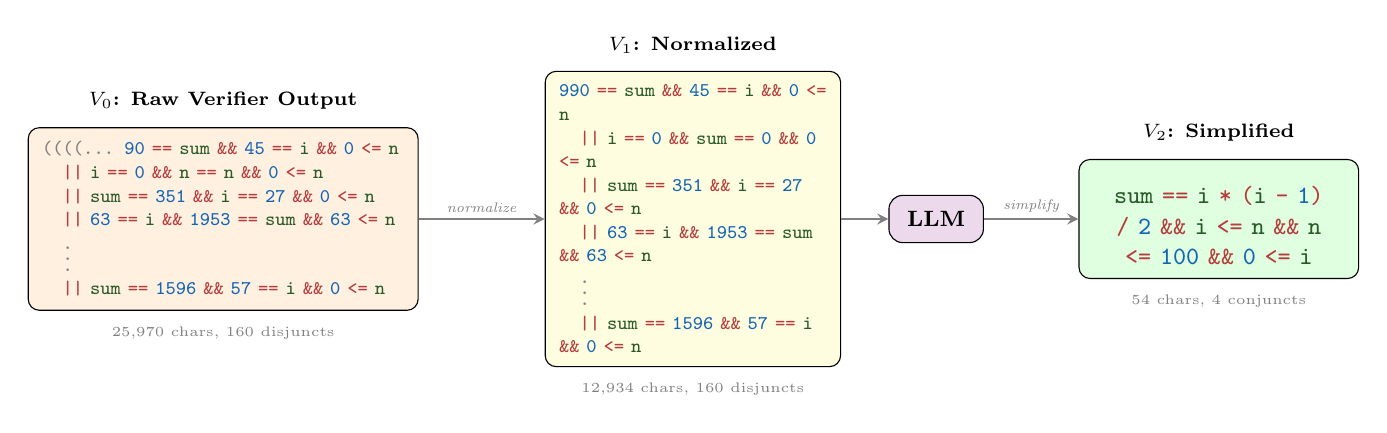
\begin{tikzpicture}[
    codebox/.style={
        draw,
        rounded corners=4pt,
        font=\ttfamily\fontsize{7}{8.5}\selectfont,
        align=left,
        fill=#1,
        inner sep=5pt
    },
    codebox/.default=white,
    llmbox/.style={
        draw,
        rounded corners=5pt,
        fill=violet!15,
        font=\footnotesize\bfseries,
        minimum height=0.6cm,
        minimum width=1.2cm
    },
    lbl/.style={font=\fontsize{7.5}{9}\selectfont\bfseries},
    sublbl/.style={font=\tiny, text=gray},
    arrowlbl/.style={font=\tiny\itshape, fill=white, inner sep=2pt}
]

% === V0: Raw Verifier Output ===
\node[codebox=orange!12, text width=4.6cm] (v0) {
\textcolor{gray}{((((...} \textcolor{num}{90} \textcolor{op}{==} \textcolor{id}{sum} \textcolor{op}{\&\&} \textcolor{num}{45} \textcolor{op}{==} \textcolor{id}{i} \textcolor{op}{\&\&} \textcolor{num}{0} \textcolor{op}{<=} \textcolor{id}{n}\\
\quad \textcolor{op}{||} \textcolor{id}{i} \textcolor{op}{==} \textcolor{num}{0} \textcolor{op}{\&\&} \textcolor{id}{n} \textcolor{op}{==} \textcolor{id}{n} \textcolor{op}{\&\&} \textcolor{num}{0} \textcolor{op}{<=} \textcolor{id}{n}\\
\quad \textcolor{op}{||} \textcolor{id}{sum} \textcolor{op}{==} \textcolor{num}{351} \textcolor{op}{\&\&} \textcolor{id}{i} \textcolor{op}{==} \textcolor{num}{27} \textcolor{op}{\&\&} \textcolor{num}{0} \textcolor{op}{<=} \textcolor{id}{n}\\
\quad \textcolor{op}{||} \textcolor{num}{63} \textcolor{op}{==} \textcolor{id}{i} \textcolor{op}{\&\&} \textcolor{num}{1953} \textcolor{op}{==} \textcolor{id}{sum} \textcolor{op}{\&\&} \textcolor{num}{63} \textcolor{op}{<=} \textcolor{id}{n}\\
\quad \textcolor{gray}{\vdots}\\
\quad \textcolor{op}{||} \textcolor{id}{sum} \textcolor{op}{==} \textcolor{num}{1596} \textcolor{op}{\&\&} \textcolor{num}{57} \textcolor{op}{==} \textcolor{id}{i} \textcolor{op}{\&\&} \textcolor{num}{0} \textcolor{op}{<=} \textcolor{id}{n}\\
};
\node[lbl, above=0.1cm of v0] {$V_0$: Raw Verifier Output};
\node[sublbl, below=0.08cm of v0] {25,970 chars, 160 disjuncts};

% === V1: Normalized ===
\node[codebox=yellow!12, text width=3.4cm, right=1.6cm of v0] (v1) {
\textcolor{num}{990} \textcolor{op}{==} \textcolor{id}{sum} \textcolor{op}{\&\&} \textcolor{num}{45} \textcolor{op}{==} \textcolor{id}{i} \textcolor{op}{\&\&} \textcolor{num}{0} \textcolor{op}{<=} \textcolor{id}{n}\\
\quad \textcolor{op}{||} \textcolor{id}{i} \textcolor{op}{==} \textcolor{num}{0} \textcolor{op}{\&\&} \textcolor{id}{sum} \textcolor{op}{==} \textcolor{num}{0} \textcolor{op}{\&\&} \textcolor{num}{0} \textcolor{op}{<=} \textcolor{id}{n}\\
\quad \textcolor{op}{||} \textcolor{id}{sum} \textcolor{op}{==} \textcolor{num}{351} \textcolor{op}{\&\&} \textcolor{id}{i} \textcolor{op}{==} \textcolor{num}{27} \textcolor{op}{\&\&} \textcolor{num}{0} \textcolor{op}{<=} \textcolor{id}{n}\\
\quad \textcolor{op}{||} \textcolor{num}{63} \textcolor{op}{==} \textcolor{id}{i} \textcolor{op}{\&\&} \textcolor{num}{1953} \textcolor{op}{==} \textcolor{id}{sum} \textcolor{op}{\&\&} \textcolor{num}{63} \textcolor{op}{<=} \textcolor{id}{n}\\
\quad \textcolor{gray}{\vdots}\\
\quad \textcolor{op}{||} \textcolor{id}{sum} \textcolor{op}{==} \textcolor{num}{1596} \textcolor{op}{\&\&} \textcolor{num}{57} \textcolor{op}{==} \textcolor{id}{i} \textcolor{op}{\&\&} \textcolor{num}{0} \textcolor{op}{<=} \textcolor{id}{n}\\
};
\node[lbl, above=0.1cm of v1] {$V_1$: Normalized};
\node[sublbl, below=0.08cm of v1] {12,934 chars, 160 disjuncts};

% === LLM ===
\node[llmbox, right=0.6cm of v1] (llm) {LLM};

% === V2: Simplified ===
\node[codebox=green!12, right=1.2cm of llm, minimum height=1.5cm, text width=3.2cm, align=center, font=\ttfamily\small] (v2) {
\vfill
\textcolor{id}{sum} \textcolor{op}{==} \textcolor{id}{i} \textcolor{op}{*} \textcolor{op}{(}\textcolor{id}{i} \textcolor{op}{-} \textcolor{num}{1}\textcolor{op}{)} \textcolor{op}{/} \textcolor{num}{2} \textcolor{op}{\&\&} \textcolor{id}{i} \textcolor{op}{<=} \textcolor{id}{n} \textcolor{op}{\&\&} \textcolor{id}{n} \textcolor{op}{<=} \textcolor{num}{100} \textcolor{op}{\&\&} \textcolor{num}{0} \textcolor{op}{<=} \textcolor{id}{i}
\vfill
};
\node[lbl, above=0.1cm of v2] {$V_2$: Simplified};
\node[sublbl, below=0.08cm of v2] {54 chars, 4 conjuncts};

% === Arrows ===
\draw[->, >=stealth, thick, gray] (v0.east) -- (v1.west) node[arrowlbl, midway, above] {normalize};
\draw[->, >=stealth, thick, gray] (v1.east) -- (llm.west);
\draw[->, >=stealth, thick, gray] (llm.east) -- (v2.west) node[arrowlbl, midway, above] {simplify};

\end{tikzpicture}
\caption{\textsc{Wonda} pipeline on \texttt{2456\_3.c}. The raw verifier output ($V_0$) is normalized ($V_1$); the LLM then extracts the triangular-number closed form and keeps only necessary loop bounds ($V_2$): \texttt{sum == i * (i - 1) / 2 \&\& i <= n \&\& n <= 100 \&\& 0 <= i}, a $481\times$ character reduction with \textbf{5.1$\times$} verification speedup.}
\label{fig:pipeline_showcase_2456_3_c}
\end{figure*}

\end{document}
